\documentclass{beamer}
\usepackage{ dsfont }
\usepackage[utf8]{inputenc}
\usepackage[english]{babel}
\setbeamersize{text margin left=10pt, text margin right=10pt} %new code
\usepackage{graphicx}
\usepackage{float}
\usepackage{subcaption}
\usefonttheme{professionalfonts} % using non standard fonts for beamer
\setbeamerfont{frametitle}{series=\bfseries}
\usepackage{animate}
\usepackage{movie15}
\usepackage{breqn, bm}
\usepackage{amsmath}
\usepackage[skins]{tcolorbox}
\usepackage{subcaption}

\definecolor{notgreen}{RGB}{255,127,0}
\definecolor{green}{RGB}{49,150,3}
\setbeamerfont{headline}{size=\small}


%----------------------------------------------------------------------------------------
%	 Package
%----------------------------------------------------------------------------------------
\usepackage{color}
\usepackage{url}
\beamertemplatenavigationsymbolsempty
\definecolor{cadmiumred}{rgb}{0.8, 0.8, 0.8}

%----------------------------------------------------------------------------------------
%	 Presentation settings
%----------------------------------------------------------------------------------------

\usetheme{default}
\usecolortheme{default}

\setbeamertemplate{itemize items}[triangle] 
\setbeamertemplate{enumerate items}[default]
 
\title[Variational Drop Out]{
	HSE Deep Learning\\ 
	\vspace{1cm}
	\textbf{\textcolor{black}{Image Captiononing}}}

\author{Ashuha Arseniy$^{1, 2}$}
\institute[Bayesgroup, MIPT]{
	Bayesian Research Group$^1$, MIPT$^2$\\
	
	\medskip
	
\includegraphics[scale=0.5]{./img/logo} 
\includegraphics[scale=0.12]{./img/mipt}
	
	\href{ars-ashuha.ru/slides}{ars-ashuha.ru/slides}}

\date{\today}

\newcommand{\Expect}{\mathsf{E}}
\newcommand{\MExpect}{\mathsf{M}}
\newcommand{\cov}{\mathsf{cov}}
\setbeamertemplate{section in toc}[circle]

\addtobeamertemplate{navigation symbols}{}{%
	\usebeamerfont{footline}%
	\usebeamercolor[fg]{footline}%
	\hspace{1em}%
	\insertframenumber/\inserttotalframenumber
}


\begin{document}
\begin{frame}
	\titlepage 
\end{frame}

\begin{frame}{Motivation}
	
	\begin{itemize}
		  \item Just for fun   \href{http://cs.stanford.edu/people/karpathy/deepimagesent/rankingdemo/}{http://cs.stanford.edu/people/karpathy/deepimagesent/rankingdemo/}
		
			\begin{center}
				  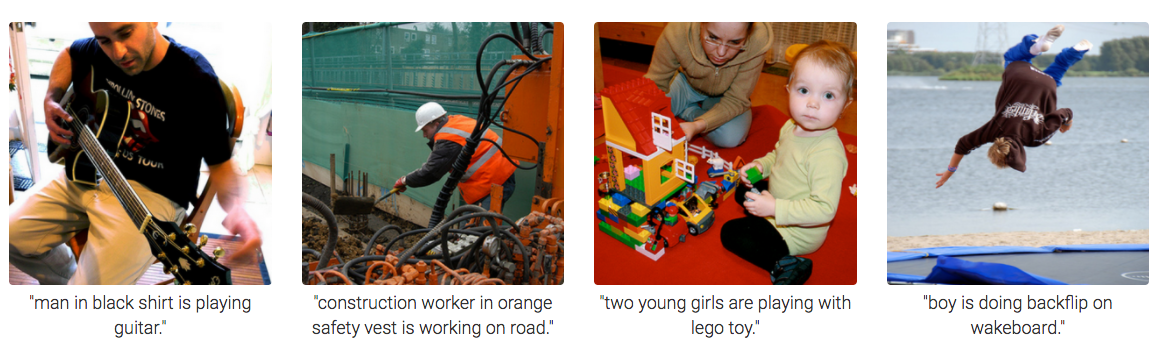
\includegraphics[scale=0.25]{img/ic} 
			\end{center}
		
		  \item Medical application
		
			\begin{center}
				  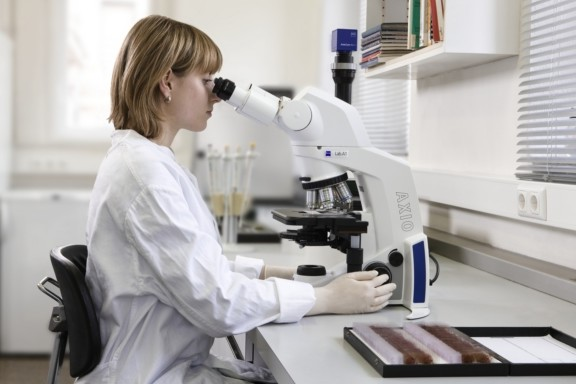
\includegraphics[scale=0.15]{img/mic}~~~
				  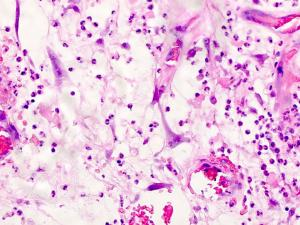
\includegraphics[scale=0.3]{img/mic2}  
			\end{center}
	\end{itemize}

\end{frame}

\begin{frame}{What should we do?}
	\begin{itemize}
		  \item We want to make image captioning
		  \item Make image description
		
			\begin{center}
				  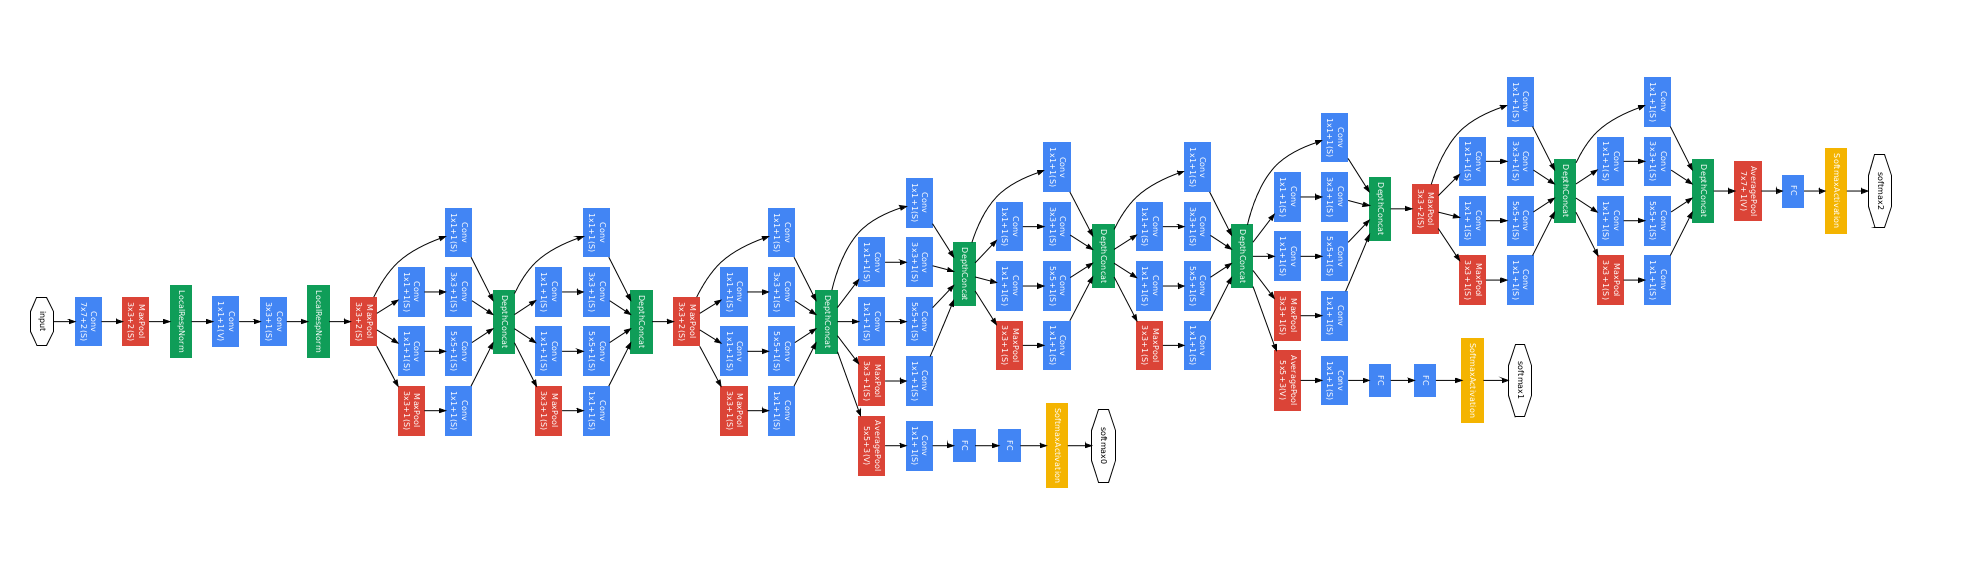
\includegraphics[scale=0.25]{img/gn}
			\end{center}
		
		  \item Make words description 
			\begin{center}
				  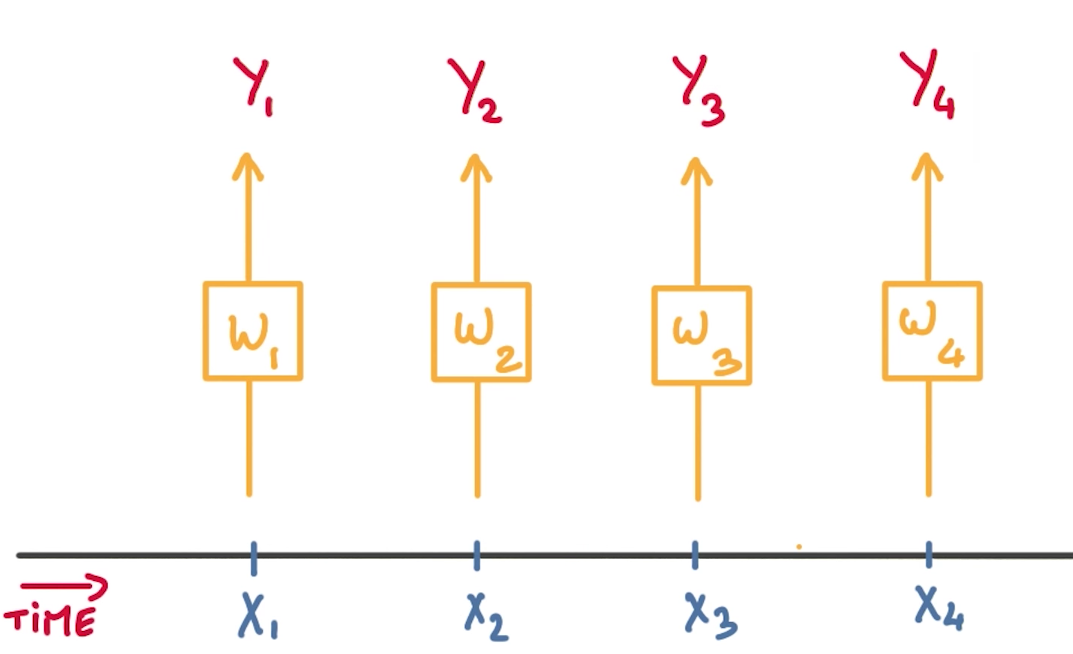
\includegraphics[scale=0.15]{img/rec}
			\end{center}
		  \item Generative Model
	\end{itemize}
\end{frame}

\begin{frame}{Convolution Neural Nets}
	\begin{itemize}
		  \item We want to make image captioning
		  \item Make image description
		
		\begin{center}
			  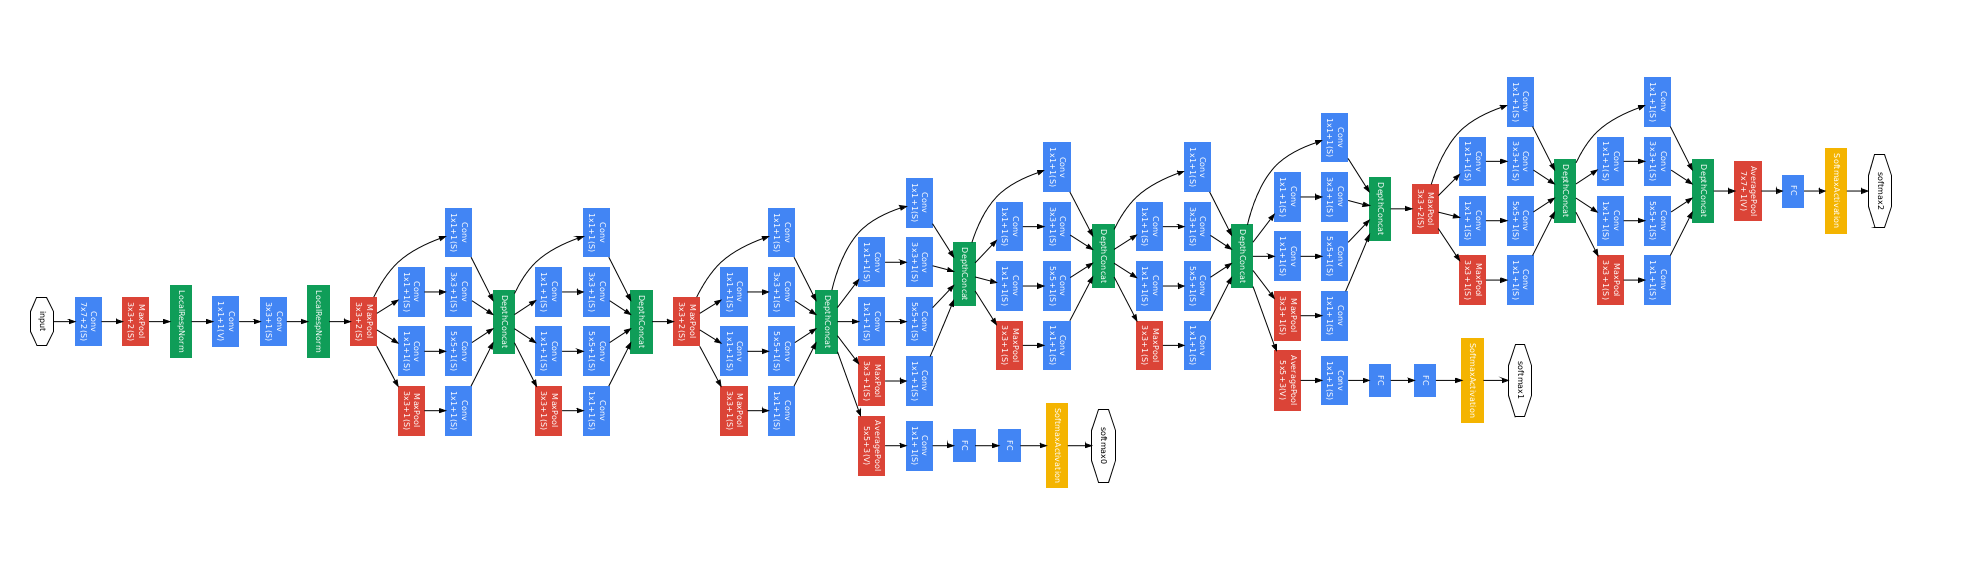
\includegraphics[scale=0.25]{img/gn}
		\end{center}
		
		  \item Make words description 
		\begin{center}
			  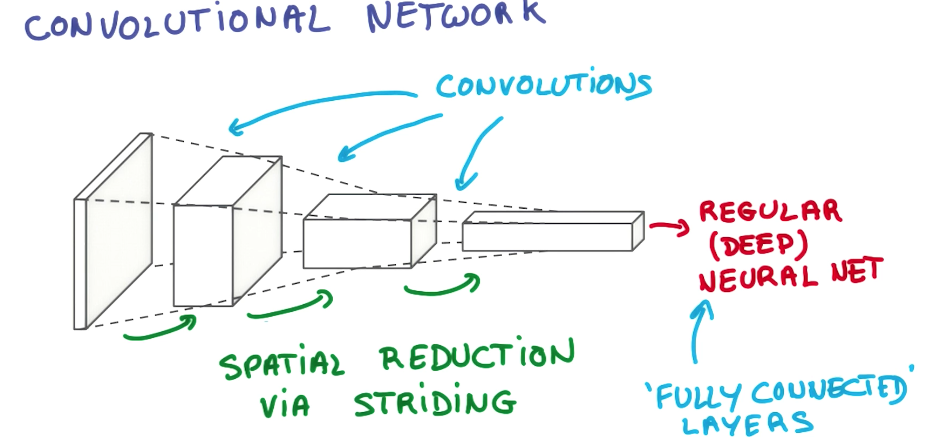
\includegraphics[scale=0.15]{img/cnn}
		\end{center}
		  \item Generative Model
	\end{itemize}
\end{frame}


\begin{frame}{Recurrent Neural Nets}
	\begin{itemize}
		  \item Conception
		
		\begin{center}
			  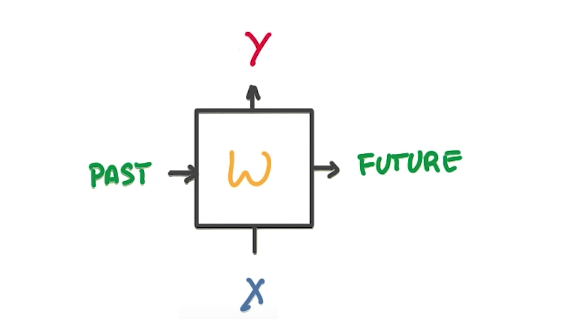
\includegraphics[scale=0.3]{img/recurent}
		\end{center}
		
		  \item LSTM
		\begin{center}
			  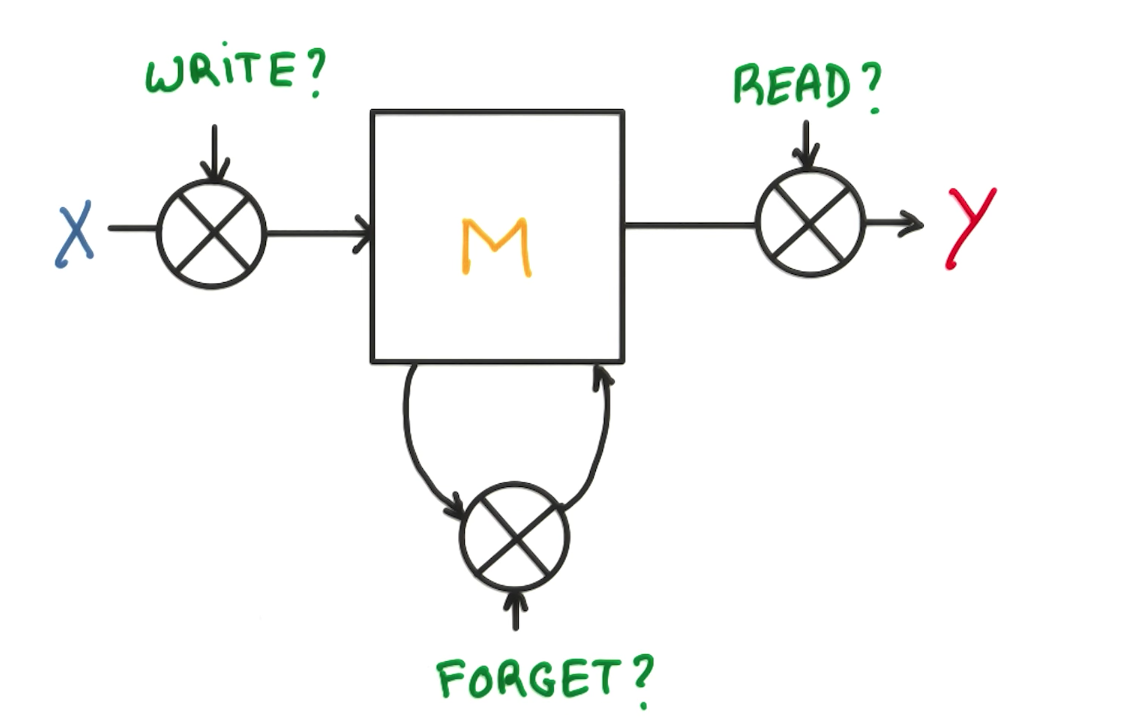
\includegraphics[scale=0.15]{img/lstm}
		\end{center}
	\end{itemize}
\end{frame}

\begin{frame}{Recurrent Neural Nets}
	\begin{itemize}
		  \item LSTM
		
		\begin{center}
			  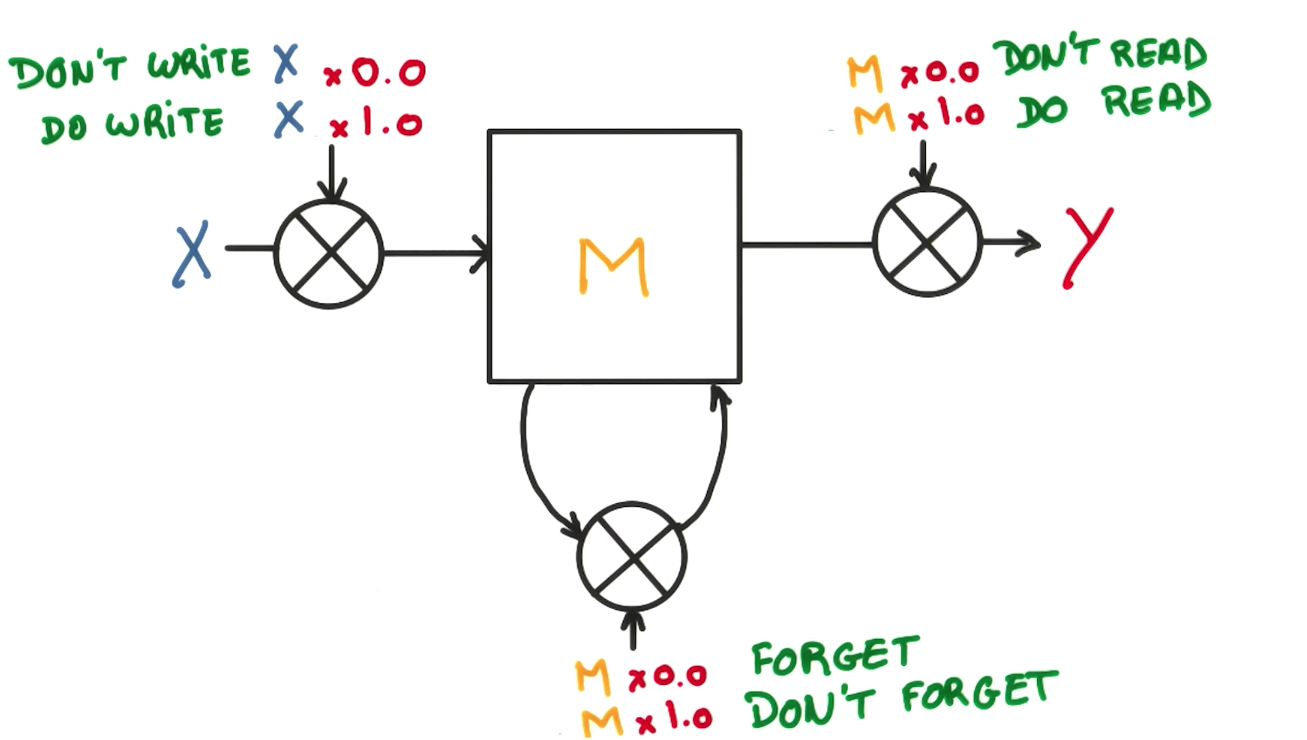
\includegraphics[scale=0.15]{img/lstm2}
		\end{center}
		
		  \item Embeding
		\begin{center}
			  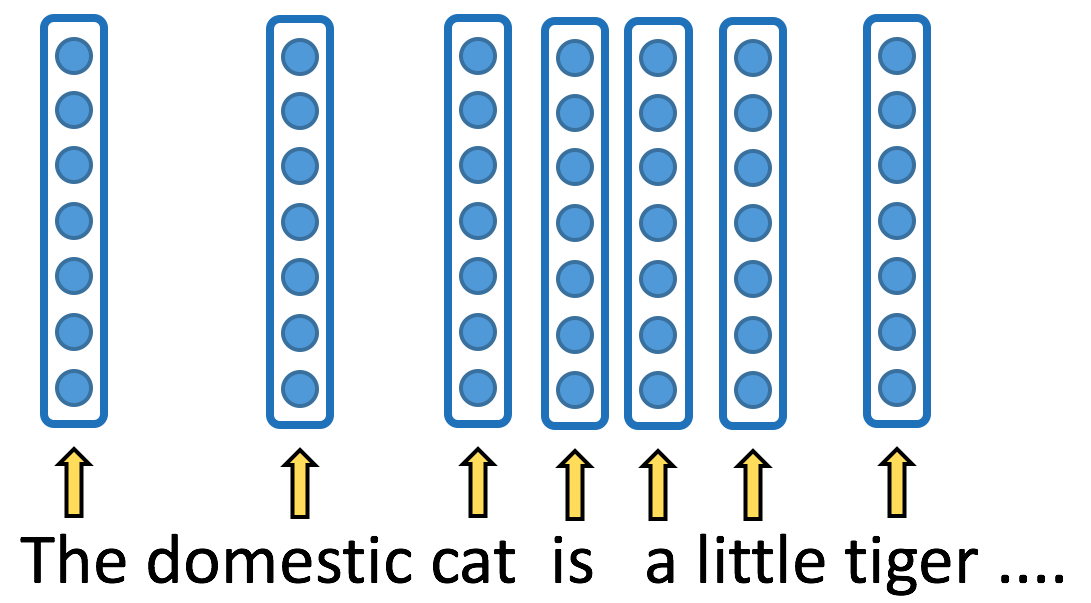
\includegraphics[scale=0.15]{img/text_repr.png}
		\end{center}
	\end{itemize}
\end{frame}

\begin{frame}{Image Captioning}
	
	\begin{itemize}
		  \item Captioning
		
		\begin{center}
			  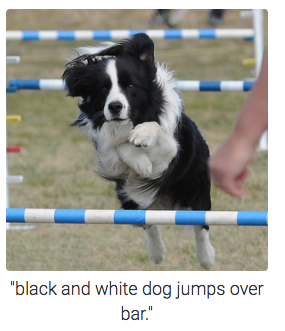
\includegraphics[scale=0.25]{img/ic2}  ~~~~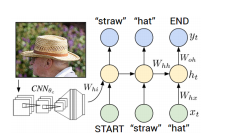
\includegraphics[scale=0.7]{img/ic3}
		\end{center}
		
		  \item Captioning?
			\begin{center}
				  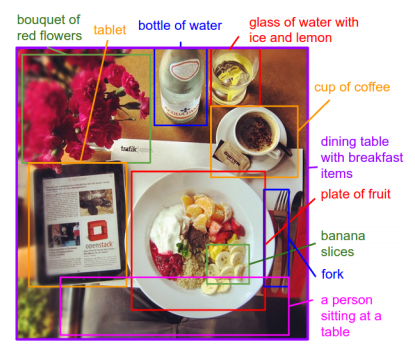
\includegraphics[scale=0.2]{img/icc}
			\end{center}
	\end{itemize}
	  \href{http://cs.stanford.edu/people/karpathy/cvpr2015.pdf}{http://cs.stanford.edu/people/karpathy/cvpr2015.pdf}
\end{frame}

\begin{frame}{Image Captioning}
	
	\begin{center}
				  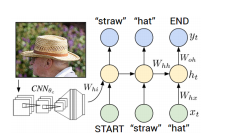
\includegraphics[scale=0.7]{img/ic3}
				
				  \href{http://mybinder.org/repo/ars-ashuha/caption_binder}{\textcolor{red}{http://mybinder.org/repo/ars-ashuha/caption\_binder}}
	\end{center}
	


\end{frame}





\end{document}

